\documentclass[a4paper, 12pt]{article}
\usepackage{graphicx}
\usepackage[UTF8]{ctex}
\usepackage{color}
\usepackage{pdfpages}
\usepackage{listings}
%文档类型(较短的文章、报告)纸张大小为A4,文字大小为12pt
%还有其他文档类型如report(更长的文档)、proc(会议论文)、book、beamer、slides
\begin{document}
	%每个文档都有一个begin{document}和end{document},两者之间是文档的主体,begin之前是文档导言区
	\title{My first Document}
	\author{肖予纯}
	\date{2024/8/25}
	\maketitle
	%锻炼顶格 \\表示换行
	\noindent	My homework \\First. Latex with 20 points. 
	\\%换行
	
	%斜体
	Some text with \emph{emphasis and \emph{nested} context}%可嵌套使用
	
	Some text with \textit{italic and \textit{nested} context}%不可嵌套使用
	\\
	\textsl{words slanted}\\
	%小号的大写字母
	\textsc{words in smallcaps}\\
	%加黑
	\textbf{words in bold}\\
	%电传机的字体
	\texttt{words in teletype}\\
	%罗马字体
	\textrm{roman words}\\
	%下划线字体
	\underline{underlined words}\\
	
	%使用颜色
	{\color{red}words are red}
	\colorbox{green}{colorbox is green}
	\colorbox{yellow}{{\color{red}words are red and box is yellow}}
	%字体大小
	\\
	normal size
	{\tiny tiny size}\\
	{\scriptsize script size}\\
	{\footnotesize footnote size}\\
	{\small small size}\\
	{\large large size}\\
	{\Large Large size}\\
	{\LARGE LARGE size}\\
	{\huge huge size}\\
	%特殊字符,为了使用这些字符,需要在他们前面添加反斜杠进行转义
	特殊字符:
	\# \$ \% \^{} \& \_ \{ \} \~{}
	
	%章节
	\section{Title of the first section}
	\subsection{Subsection of the first section}
	\subsubsection{subsection of the first subsection}
	\paragraph{paragraph one}
	\section{Second section}
	%表格
	\begin{tabular}{|l|l|}
		Apples       & Green  \\% 符号'&'用于分割列
		\cline{1-1}Strawberries & Red    \\
		Orange       & Orange \\
	\end{tabular}
	\\
	\begin{tabular}{rc}
		Apples              & Green  \\
		\hline  %分割行
		Strawberries        & Red    \\
		\cline{1-2} Oranges & Orange \\ %在第一列和第二列之间插入横线
	\end{tabular}
	%列表
	\\
	\\two kinds of list:
	\begin{enumerate}
		\item An entry
		\item Another One
		\item Wow! Three entries
	\end{enumerate}
	\begin{itemize}
		\item An entry
		\item[-] Another One
		\item[+] Wow! Three entries
		\item[A] ‘A’作为标号
	\end{itemize}
	%插入图片
	\begin{figure}[h]
		\centering
		
\includegraphics[width=1\textwidth]{image}
		\caption{Here is my image}
		\label{image-myimage}
	\end{figure}
	%插入公式
	$1+2=3$
	$$1+2=3$$\\%有行间的公式
	%有标号的公式
	\begin{equation}
		1+2=3
	\end{equation}
	%数学符号
	$n^2$\\%上标
	$2_a$\\%下标
	$b——{a-2}$\\%上、下标含有多个字符
	$$\frac{a}{3}$$\\%分数,可嵌套
	$$\sqrt{y^2}$$\\%根号
	$$\sqrt[x]{y^2}$$\\
	$$\sum_{x=1}^5 y^z$$\\%求和
	$$\int_a^b f(x)$$\\%积分
	%希腊字母
	$\aleph$
	$\beta$
	$\delta$
	$\Delta$
	$\pi,\Pi$
	\\这是我引用的第一篇文献\cite{1284395}。\\
	第二篇\cite{10335618}\\
	\cite{666}
	\newpage
	%插入文献
	\bibliographystyle{unsrt}
	\bibliography{reference}
	
	%导入pdf
	%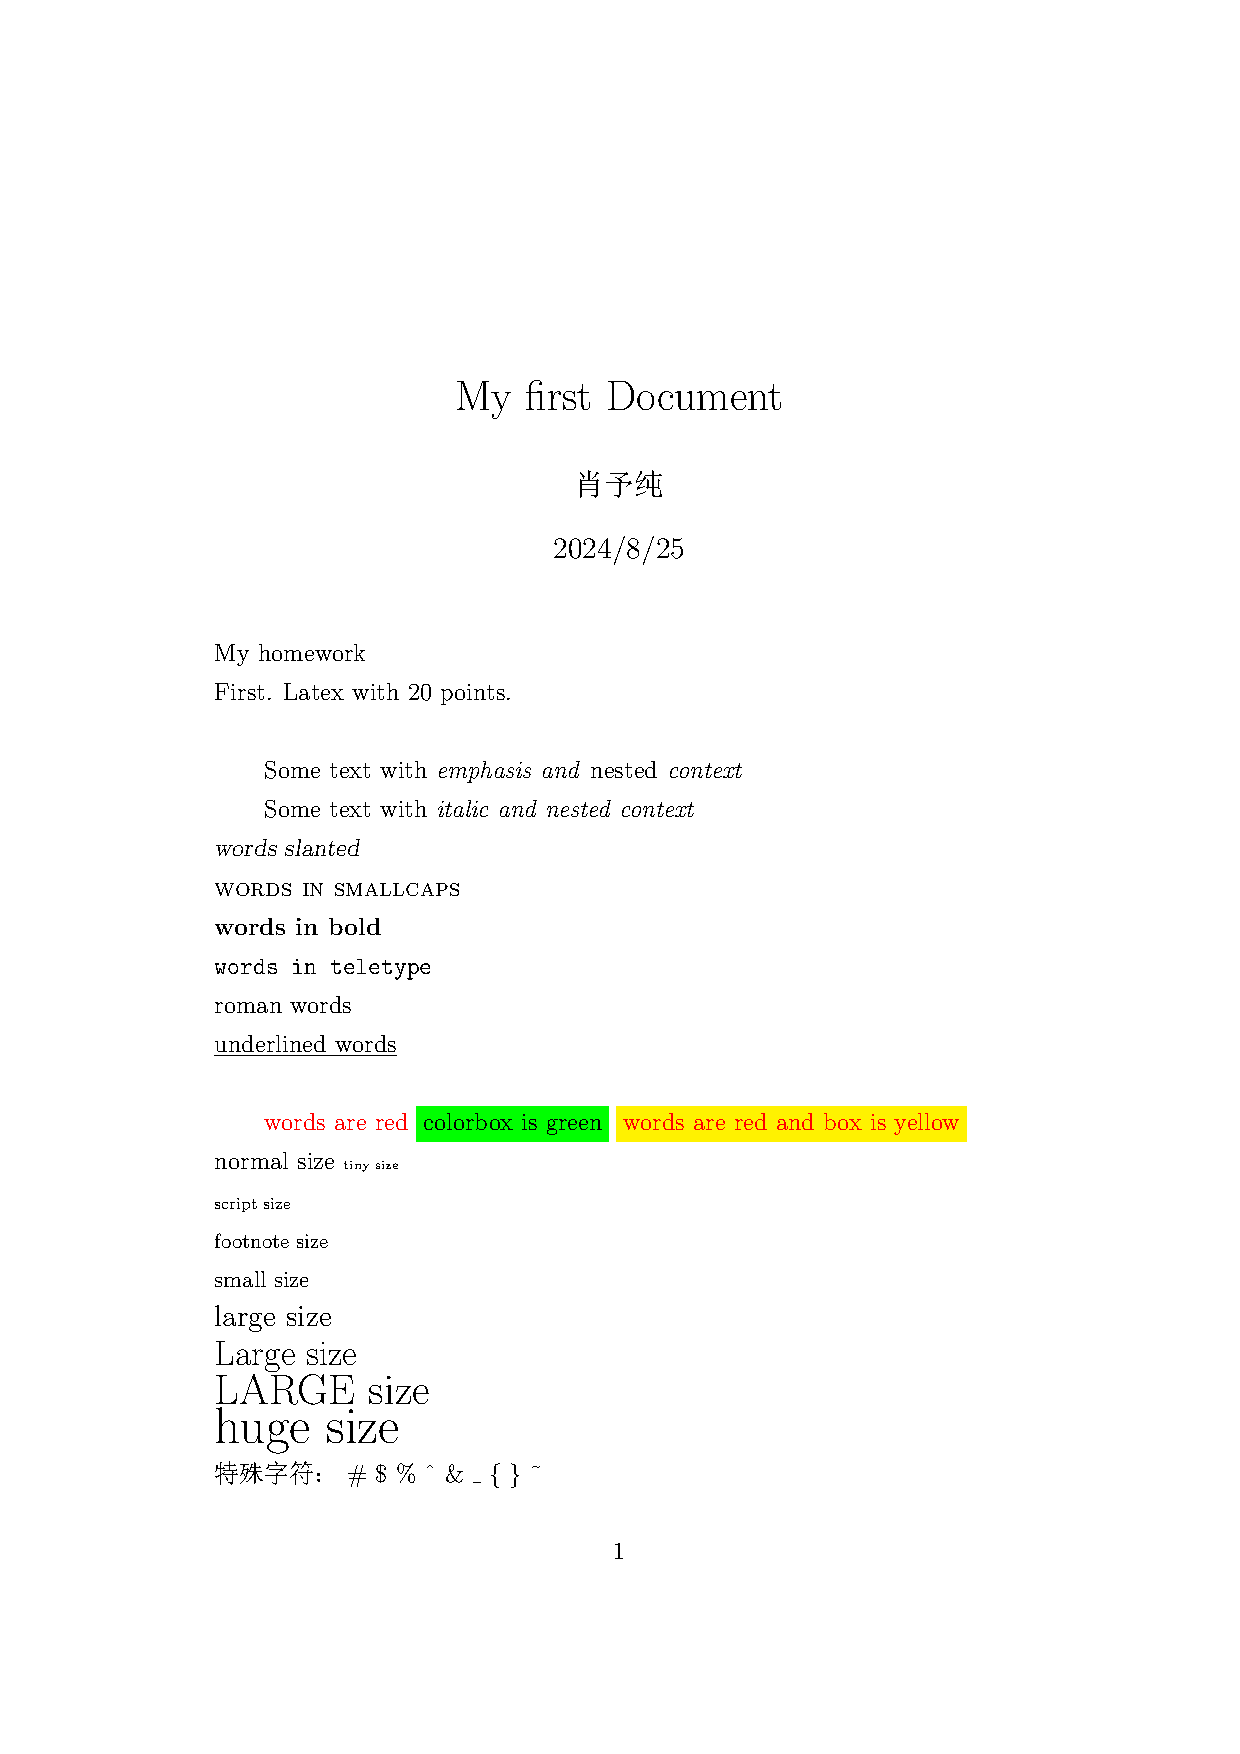
\includepdf{document.pdf}
	
	%插入代码块
	附上代码块:
	\begin{lstlisting}
		#include <iostream>
		using namespace std;
		
		int main()
		{
			cout<<"hello"<<endl;
			return 0;
		}
	\end{lstlisting}
\end{document}